\documentclass[12pt]{article}


\usepackage{amssymb}
\usepackage{amsmath}
\usepackage[utf8]{inputenc}
%\usepackage[ngerman]{babel}
\usepackage{lineno}
\usepackage{listings}
\usepackage[T1]{fontenc}
\usepackage[utf8]{inputenc}
\usepackage{lmodern}
\usepackage{eurosym}
\usepackage{listings}
\usepackage{microtype}
\usepackage{units}
\usepackage{color}
\usepackage{xcolor}
\usepackage{graphicx}
\usepackage{subfigure}
\usepackage{import}
\usepackage{url}
\usepackage{amsthm}
\theoremstyle{plain}

\lstset
{ %
  language=R,                     % the language of the code
  basicstyle=\footnotesize\ttfamily,       % the size of the fonts that are used for the code
  numbers=left,                   % where to put the line-numbers
  numberstyle=\tiny\color{gray},  % the style that is used for the line-numbers
  stepnumber=1,                   % the step between two line-numbers. If it's 1, each line
                                  % will be numbered
  numbersep=5pt,                  % how far the line-numbers are from the code
  backgroundcolor=\color{white},  % choose the background color. You must add \usepackage{color}
  showspaces=false,               % show spaces adding particular underscores
  showstringspaces=false,         % underline spaces within strings
  showtabs=false,                 % show tabs within strings adding particular underscores
  frame=single,                   % adds a frame around the code
  rulecolor=\color{black},        % if not set, the frame-color may be changed on line-breaks within not-black text (e.g. commens (green here))
  tabsize=2,                      % sets default tabsize to 2 spaces
  captionpos=b,                   % sets the caption-position to bottom
  breaklines=true,                % sets automatic line breaking
  breakatwhitespace=false,        % sets if automatic breaks should only happen at whitespace
  title=\lstname,                 % show the filename of files included with \lstinputlisting;
                                  % also try caption instead of title
%  keywordstyle=\color{blue},      % keyword style
%  commentstyle=\color{green},   % comment style
%  stringstyle=\color{blue},       % string literal style
  %escapeinside={\%*}{*)},         % if you want to add a comment within your code
  escapeinside={(*@}{@*)},         
  morekeywords={*,...}            % if you want to add more keywords to the set
} 

\title{\vspace{-2cm}NetSec: Blatt 4}
\author{Jonas Sander \\ Kolja Hopfmann \\UHH SoSe18}
\date{\today}

\begin{document}
\pagenumbering{arabic}
\maketitle
\centerline{\rule{1.2\linewidth}{.2pt}}
%\shorthandoff{"}
\section{Vertrautmachen mit der Umgebung}
Die VMs wurden in der angegebenen Reihenfplge gestartet, auf SurfingVM und RouterVM wurde der Benutzer user/user angemeldet. Mit dem Befehl $/sbin/ifconfig$ wurden die Daten erhalten:\\
SurfingVM:\\
ip-Adresse: 192.68.254.44\\
Gateway: 192.68.254.1\\
DNS-Server: 10.1.1.1\\
RouterVM:\\
ens33 IP: 172.16.65.139\\
ens36 IP: 192.168.254.1\\
Gateway: 172.16.65.2\\
Der Ping zu 10.1.1.1 war erfolgreich unter surfen im Internet möglich, der Ping zu 10.1.1.2 war nicht erfolgreich, da der Server nicht verfügbar war.
\section{Sniffing mit tcpdump}
sudo tcpdump -p -i any host 192.168.254.44 or 10.1.1.1\\
Mit diesem Befehl wurde, alle Nachrichten protokolliert, die von der SurfingVM gesendet oder empfangen werden. 
Die Felder, die in einer DNS-Antwort übertragen werden sehen wie folgt aus:\\
<timestamp> IP <source IP-Adress and port> > <destination IP Adress and port> Flags [<flags>] <sequence from to, ack number| ack> <tcp window> <packet length>\\
Ausgabe siehe Anhang.
\begin{itemize}
\item
sudo tcpdump -p -i any src 192.168.254.44 or 10.1.1.1 and port 80\\
Durch die Einschränkung auf Port 80 wir nurnoch der HTTP Verkehr protokolliert, Ausgabe siehe Anhang.
\item
sudo tcpdump -p -A -i any src 192.168.254.44 or 10.1.1.1 and port 80\\
Dur das -A Flag derden die Protokollierten Pakete als Ascii-Code angezeigt. Die Pakete sind vermutlich zu groß als dass tcpdump sie komplett abfängt.\\
sudo tcpdump -p -A -nnvvSs 65535 -i any src 192.168.254.44 or 10.1.1.1 and port 80\\
Durch die -nnvvSs Flag werden pro Paket nun bis zu 65535 Byte Protokolliert.
%TODO: snippets aus dem Anhang vergleichen
Ausgaben siehe Anhang
\item
%TODO: snippets aus dem Anhang einfügen
Der Header ist Base64 Codiert. 
\end{itemize}
\section{Sniffing mit dsniff und urlsnarf}
\subsection{}
\begin{itemize}
\item sudo urlsnarf -i any -v ".*" src 192.168.254.44 or 10.1.1.1 and port 80
\end{itemize}
Urlsnarf wird ausgeführt, sodass auf alle Netwerk-Interfaces gesnifft wird. Source IP-Adresse ist die SurfingVM oder der DNS-Server. So wird der Gesamte HTTP-Verkehr zwischen den beiden aufgezeichnet.
\subsection{}
\begin{itemize}
\item sudo dsniff -i any src 192.168.254.44 or 10.1.1.2
\end{itemize}
Dsniff sucht in der Kommunikation von SurfingVM und Laborserver nach entschlüsselbaren Passwörtern
\section{Sniffing mit Wireshark}
Ein Capture-Filter gibt an, welche Pakete von Wireshark erfasst werden sollen. Capture-Filter werden immer am Anfang einer Capture-Session festgelegt. \\ \\
Ein Display-Filter ist lediglich ein visueller Filter auf allen erfassten Paketen uns kann innerhalb einer Session angepasst werden.
\\\\
Um den gesamten Traffic der SurfingVM zu protokollieren wird der Capture-Filter auf das Interface "ens36" gesetzt. Da ens36 das Router-Interface für die SurfingVM ist. Alternativ kann man auch einen Display-Filter mit "ip.src==192.168.254.44 or ip.dst==192.168.254.44" setzen. \\ \\
Nach den erstmaligen anpingen des Laborservers werden folgende Nachrichten ausgetauscht: 
\begin{itemize}
\item DNS-Server(10.1.1.1) löst Namespace "labservervm.svslab" zu 10.1.1.2 als Ziel-Adresse auf.
\item Ping-Request der SurfingVM und Ping-Response des Laborservers.
\item Auflösung der IP-Adresse zu MAC-Adresse mittels ARP.
\end{itemize}
Aus dem Ping-Command wird deutlich das die Time To Life(ttl) 127 Sekunden beträgt.
Der DNS-Server speichert den Namensraum dementsprechend lange. \\ \\
Nach Erwartung würde nun ein erneuter Ping deutlich schneller sein, da die Auflösung gespeichert ist. Tatsächlich ergab sich bei einem erneuten Ping kein Unterschied in Zeit und Art der Nachrichten. Vermutung: der DNS-Server verwendet für das Ping-Protokoll kein Caching. \\ \\
Beim Aufrufen des Laborservers mittels Web-Broswer wird das Caching nun deutlich:
Die erste Anfragen dauern ungefähr 6-12ms. Ein erneuter Aufruf der URL dauert 3ms. Am schnellsten ist der Refresh auf den Zur verfügung gestellten Link und der Refresh mit der F5-Taste mit jeweils 2ms.
\\\\
Um nun ausschließlich den HTTP-Verkehr der SurfingVM zu untersuchen wird folgender Filter verwendet: \\
(ip.dst==192.168.254.44 or ip.src==192.168.254.44) and (http and !ocsp)\\ \\
Um den HTTP-Nachrichtenaustausch näher zu untersuchen wurde die Funktion "open TCP-Stream" verwendet: \\
Rechtsklick auf HTTP package: Follow => TCP Stream => TCP Stream öffnet sich.
\\\\
Um den Traffic des TCP-Chats zu protokollieren wird folgender Display-Filter verwendet: \\
(ip.dst==192.168.254.44 or ip.src==192.168.254.44) and tcp\\\\
Beim Austausch einiger Nachrichten zwischen SurfingVM und RouterVM mittels TCP-Chats:
Das TCP-Paket vom Client(SurfingVM)\\
Der Pseudo-"Broadcast" des Chat-Servers an alle angeschlossenen Clients(hier: die SurfingVM).
Das ACK bei Beendigung der Kommunikation.
\\\\
Beim Aufruf einer Seite mit HTTPS protokolliert Wireshark Nachrichten mit dem OCSP-Protokoll ausgetauscht. Welches ein Protokoll für Sicherheitszertifikate ist.
\section{ARP-Spoofing}
sudo arpspoof 172.16.65.2\\
Die Angegebene Adresse ist das Gateway der RouterVM, arpspoof leitet nun den Gesamten Datenverkehr dorthin um.
Dieser Datenverkehr wurde ein paar Minuten lang protokolliert und anschließend in Wireshark mit $ip.addr\ == 10.1.1.2 \&\& icmp$ gefiltert, wodurch genau die Kommunikation über das Ping-Protokoll mit 10.1.1.2 angezeigt wird. Von der IP-Adresse 172.16.65.138 kam alle 37 Sekunden ein Ping, dies ist also die Adresse der MysteryVM.\\
Der Mail-Client verwendet POP, die Zugangsdaten sind User: bumblebee, Passwort: Optimus Prime. Eine sichere Alternative wäre IMAPS, welches bereits bei Verbindungsaufbau eine SSL verschlüsselung verwendet. Eine Weitere Möglichkeit wäre die Verwendung von SMTP mit eine PGP Verschlüsselung.\\
Die MysteryVM verwendet für ihre HTTP requests Mozilla Firefox 5.0 auf Ubuntu-Linux. Die Abgerufene URL ist 10.1.1.2, die Logindaten sind User: admin, Passwort: geheim. Beim Aufruf der Webseite ergibt sich kein Widerspruch.
\section{Scanning mit nmap}
\section{OpenVAS}
Dienste von OpemVAS laufen problemlos bei Überprüfung. \\
Es wird sich mit user/user auf 127.0.0.1 angemeldet. \\ \\
Bei Quick-Scan auf localhost werden 3 high severity Schwachstellen gefunden:\\
- SSL/TLS: Report Vulnerable Cipher Suites for HTTPS (2x)\\
- SSL/TLS: Certificate Signed Using a weak signature Algorithm\\\\
Scan auf MysteryVM findet OpenVAS die Zugangsdaten des SSH-Servers: root/password\\
Scan mit SSH-Credentials enthüllt enorme Anzahl an high severity Schwachstellen, wobei die Meisten davon auf eine veraltete OS-Version zurückzuführen sind.
\newline
\section{Quellen}
\begin{thebibliography}{50}
\bibitem  [Cyberciti], \url{www.cyberciti.biz/faq/how-to-find-out-default-gateway-in-ubuntu/}
\bibitem [Stackexchange] , \url{unix.stackexchange.com}
\bibitem [Tcpdump], \url{packetpushers.net/masterclass-tcpdump-interpreting-output/}
\bibitem [Wireshark], \url{wiki.wireshark.org/DisplayFilters}
\bibitem [Nmap 1], \url{ubuntuusers.de/nmap}
\bibitem [Nmap 2], \url{garron.me/en/go2linux/wich-service-or-program-listenung-port.html}
\bibitem [OpenVAS], \url{openvas.org/setup-and-start.de}
\bibitem [ARP Spoof], \url{https://en.wikipedia.org/wiki/ARP_spoofing}
\bibitem [DNS], \url{https://en.wikipedia.org/wiki/Name_server#Caching_name_server}
\bibitem [DNS 2], \url{https://en.wikipedia.org/wiki/Multicast_DNS}
\bibitem [POP], \url{https://de.wikipedia.org/wiki/Post_Office_Protocol}
\bibitem [IMAP], \url{https://de.wikipedia.org/wiki/Internet_Message_Access_Protocol}
\bibitem [SMTP], \url{https://de.wikipedia.org/wiki/Simple_Mail_Transfer_Protocol}
\bibitem [Nmap 3], \url{https://de.wikipedia.org/wiki/Nmap}	
\end{thebibliography}
\newpage
\section{Anhang}
\subsection*{Wireshark}
\subsubsection*{TCP-Chat}
\begin{figure}[!ht]
	\centering
     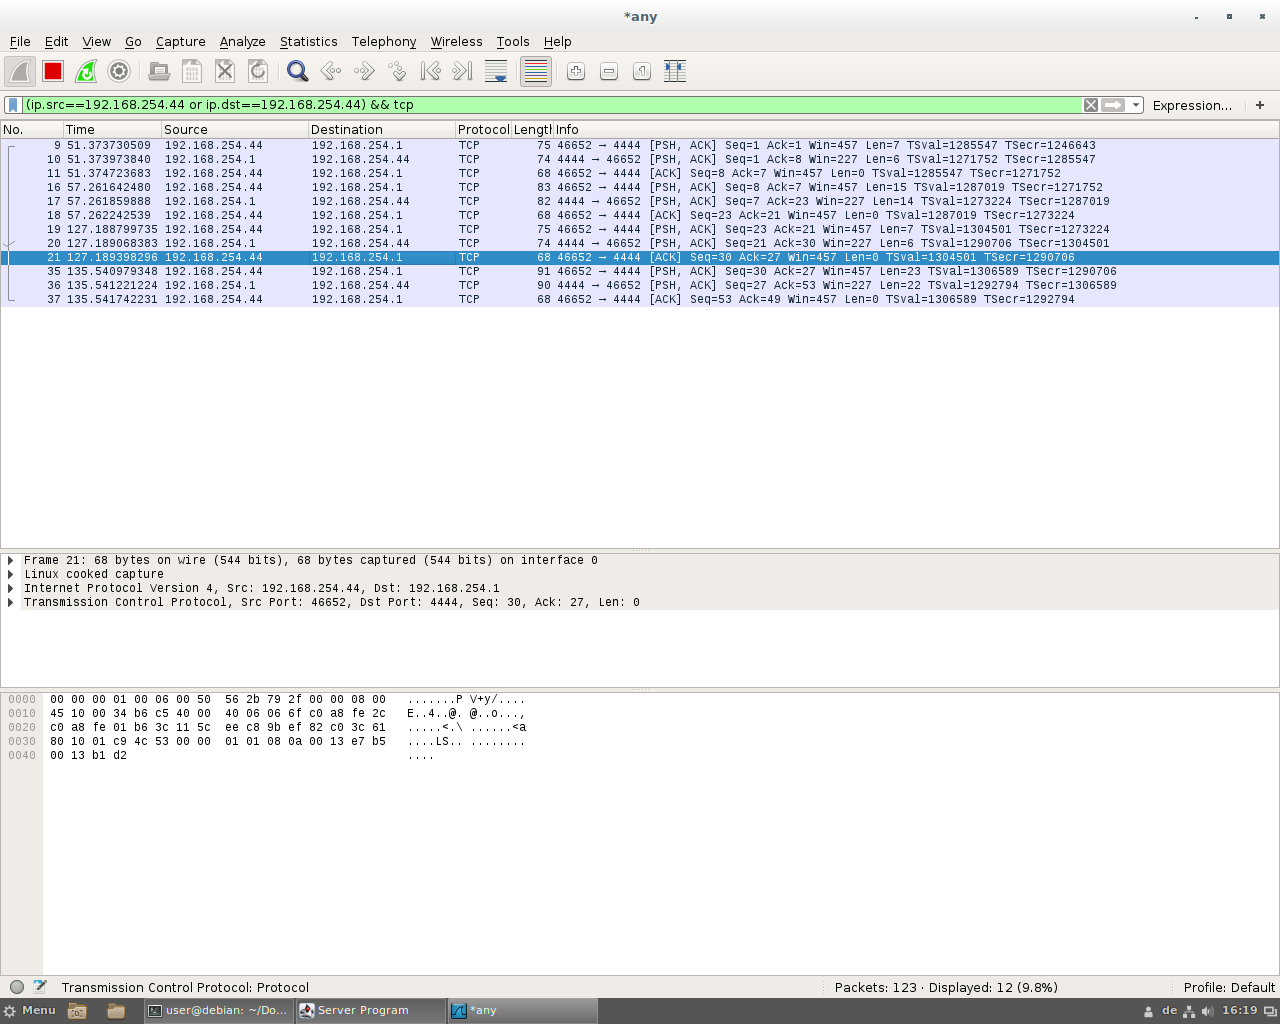
\includegraphics[width=0.9\textwidth]{Bilder/tcp-chat_1.png}
\end{figure}
\newpage
\subsubsection*{HTTPS-Traffic der SurfingVM}
\begin{figure}[!ht]
	\centering
     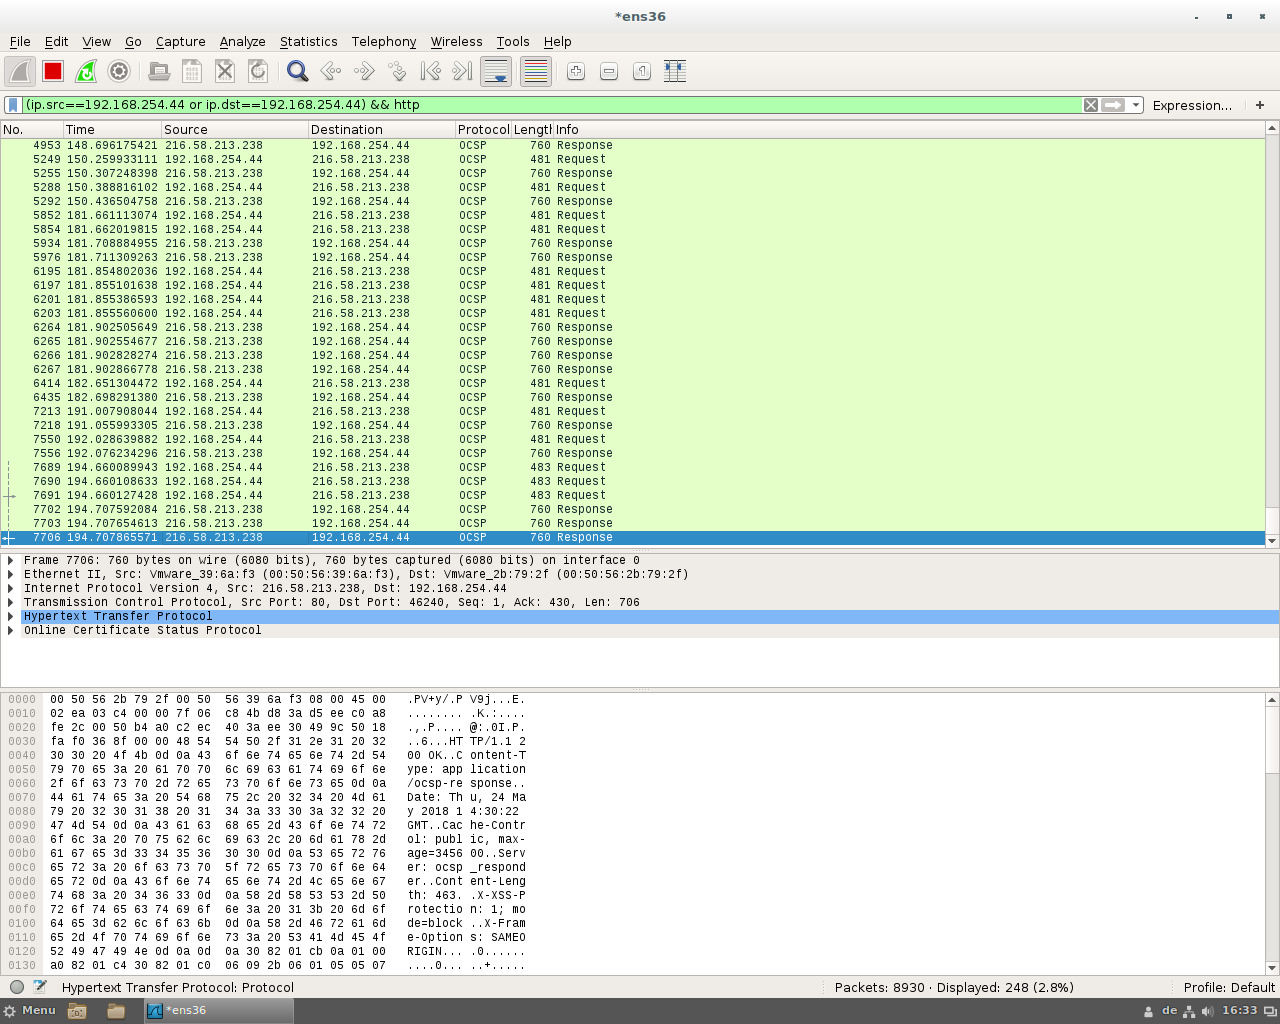
\includegraphics[width=0.9\textwidth]{Bilder/https_traffic_surfingvm.png}
\end{figure}
\end{document}
